\documentclass[a4paper,12pt,italian]{article}

% pacchetti------------------------------
% pacchetti
\usepackage[utf8]{inputenc} 
\usepackage[italian]{babel}
\usepackage{url}
\usepackage{hyperref}
\usepackage{xcolor}
%\usepackage{nopageno} % per togliere il numero delle pagine
\usepackage{graphicx} % per le immagini
\usepackage{amsthm}
\usepackage{amsmath}
\usepackage{amssymb}
\usepackage{wrapfig} % per le immagini incorniciate con il testo
\usepackage{fancyhdr} % per i headings e footers
\usepackage[backend=biber, style=numeric, defernumbers, sorting=none]{biblatex} % per la bibliografia e la sitografia
\usepackage{eurosym} % per il simbolo dell'euro "€" più carino
\usepackage{appendix}
\usepackage{geometry}
\usepackage{extpfeil}
\usepackage{tikz}
\usepackage{multirow}


% \title{Calcolo differenziale e applicazioni alla fisica\\
% \\\vspace{8pt} {\large \sc su come funzionano le pale eoliche}\\
% \vspace{32pt} {\Large Elaborato per l'Esame di Stato}\\
% \vspace{16pt}}
% \author{\sc Leandro Ye}
% \date{31 maggio 2021}

% impostazioni del pacchetto fancyhdr
\pagestyle{fancy}
\fancyhf{}
\rhead{\sc leandro ye}
\lhead{Misura del momento di inerzia di un disco}
\fancyfoot[c]{\thepage}

% impostazioni del pacchetto eurosym
\DeclareUnicodeCharacter{20AC}{\euro}

% per indicare le fonti delle citazioni
\addbibresource{citazioni.bib}




% INIZIO DOCUMENTO ---------------------------------------
\begin{document}

%\thispagestyle{plain} % per ignorare per questa pagina le impostazioni fancy
\thispagestyle{empty} % per disattivare per questa pagina le impostazioni fancy e anche il numero della pagina

\begin{figure}[h]
    \centering
    \includegraphics[width=0.5\textwidth]{image/logo.png}
    \label{Logo}
\end{figure}

\section*{\Huge \bf Misura del momento di inerzia di un disco con il Pendolo di Maxwell}

\vspace{1.0cm}

\begin{center}
    {\large 5 Maggio 2022}
\end{center}

\vspace{0.5cm}


\begin{center}
{\large Realizzato da \textsc{Leandro Ye}}    
\end{center}

\vspace{\fill}
% Abstract

\section*{}
\addcontentsline{toc}{section}{Riassunto}
\begin{center}
\framebox{
\begin{minipage}{5 in}
\begin{center}
\vspace{0.5cm}
\section*{Riassunto}
\end{center}
\textbf{L'esperimento.} Nell'esperimento si è andato a misurare il momento di inerzia di un disco non omogeneo attraverso due metodi: metodo geometrico, analizzando principalmente la geometria del disco, e metodo dinamico, ottenendo la misura attraverso l'utilizzo del pendolo di Maxwell.\\

\noindent \textbf{Risultato.} Nell'esperimento il valore del momento d'inerzia ottenuto attraverso il metodo geometrico è $I_G=(4.91 \pm 0.08) \cdot 10^{-4} \textrm{ kg} \cdot \textrm{m}^2$, mentre per il metodo dinamico è $I_D=(5.1 \pm 0.2) \cdot 10^{-4} \textrm{ kg} \cdot \textrm{m}^2$, per cui si è potuto affermare che i due valori ottenuti sono compatibili entro l'errore.
\vspace{0.5cm}
\end{minipage}}
\end{center}


\newpage

% Intro
\section*{Introduzione}
\addcontentsline{toc}{section}{Introduzione}
% Introduzione
In questo esperimento si è cercato di misurare il momento di inerzia di un oggetto: ciò si basa sul fatto che il momento d'inerzia può essere ricavato sia dalla geometria dell'oggetto e sia dal suo comportamento nel moto traslarotatorio.
Ogni corpo possiede un fattore di resistenza ad moto rotatorio attorno ad un asse, fattore che in questo caso corrisponde al suo \textbf{momento d'inerzia}.\\
Per esempio un punto materiale di massa $m$ che ruota attorno ad punto distante $r$ ha momento d'inerzia 
$$I = m r^2$$
Oppure, considerato un corpo rigido cilindrico che ruota attorno alla sua asse, con raggio $r$ e massa $m$, si può dimostrare$^{\textrm{\cite{meccanica}}}$ che possiede
$$I =  \frac{1}{2} m r^2$$
come momento d'inerzia.\\
L'aspetto fondamentale che ci permette di ricavare il valore del momento di inerzia è la sua \textbf{additività}: se un corpo rigido è composto da $n$ parti, il momento d'inerzia totale del corpo  è dato dalla \textit{somma dei momenti d'inerzia delle $n$ parti} che costituiscono il corpo, calcolati tutti rispetto allo stesso asse di rotazione.\\
Nell'esperimento il corpo in questione è un disco non omogeneo composto da quattro toroidi concentrici (Fig. \ref{disco}), quindi il momento d'inerzia ricavato mediante procedura geometrica equivale alla somma dei momenti d'inerzia dei quattro toroidi.\\

Alternativamente, è possibile ricavare il suo momento d'inerzia a seconda di come si muove dinamicamente il corpo. Infatti, attraverso l'apparato del Pendolo di Maxwell, il disco assume inizialmente una posizione ad una altezza stabilita, e una volta lasciata libera questo comincia a calare di quota assumendo un moto rototraslatorio, quindi acquistando nello stesso tempo sia energia cinetica traslatoria e sia quella rotazionale, fino ad arrivare a quota zero. Dal momento che \textit{l'energia cinetica rotazionale di un corpo rigido è direttamente proporzionale al suo momento d'inerzia}, si deduce che è possibile ricavare il valore a partire dalla \textbf{legge di conservazione dell'energia meccanica}. Infatti, un corpo rigido ha energia cinetica rotazionale $K_r$ corrispondente a
$$\displaystyle K_r = \frac{1}{2} I \omega ^2$$
con $I$ il momento d'inerzia del corpo e $\omega$ la velocità angolare rispetto all'asse di rotazione.



% 1. Metodo sperimentale
\section{Metodo sperimentale}
In questo paragrafo verranno trattati la strumentazione utilizzata, i metodi di misurazione e le formule utilizzate per il calcolo indiretto.

%%%%% 1.1 Apparato sperimentale
    \subsection{Apparato sperimentale}

    Gli strumenti utilizzati per questo esperimento sono stati:
\begin{itemize}
    \item Il \textbf{pendolo di Maxwell} (Fig. \ref{pendolo_di_maxwel}), composto da quattro oggetti fondamentali: un piedistallo, un'impalcatura, due fili e il disco di cui misurare il momento d'inerzia.
    \item Il \textbf{disco non omogeneo} di plastica (Fig. \ref{disco}), composto da quattro toroidi concentrici con al centro il perno metallico appeso ai fili del il pendolo di Maxwell.
     \begin{figure}[htbp]
        \centering
        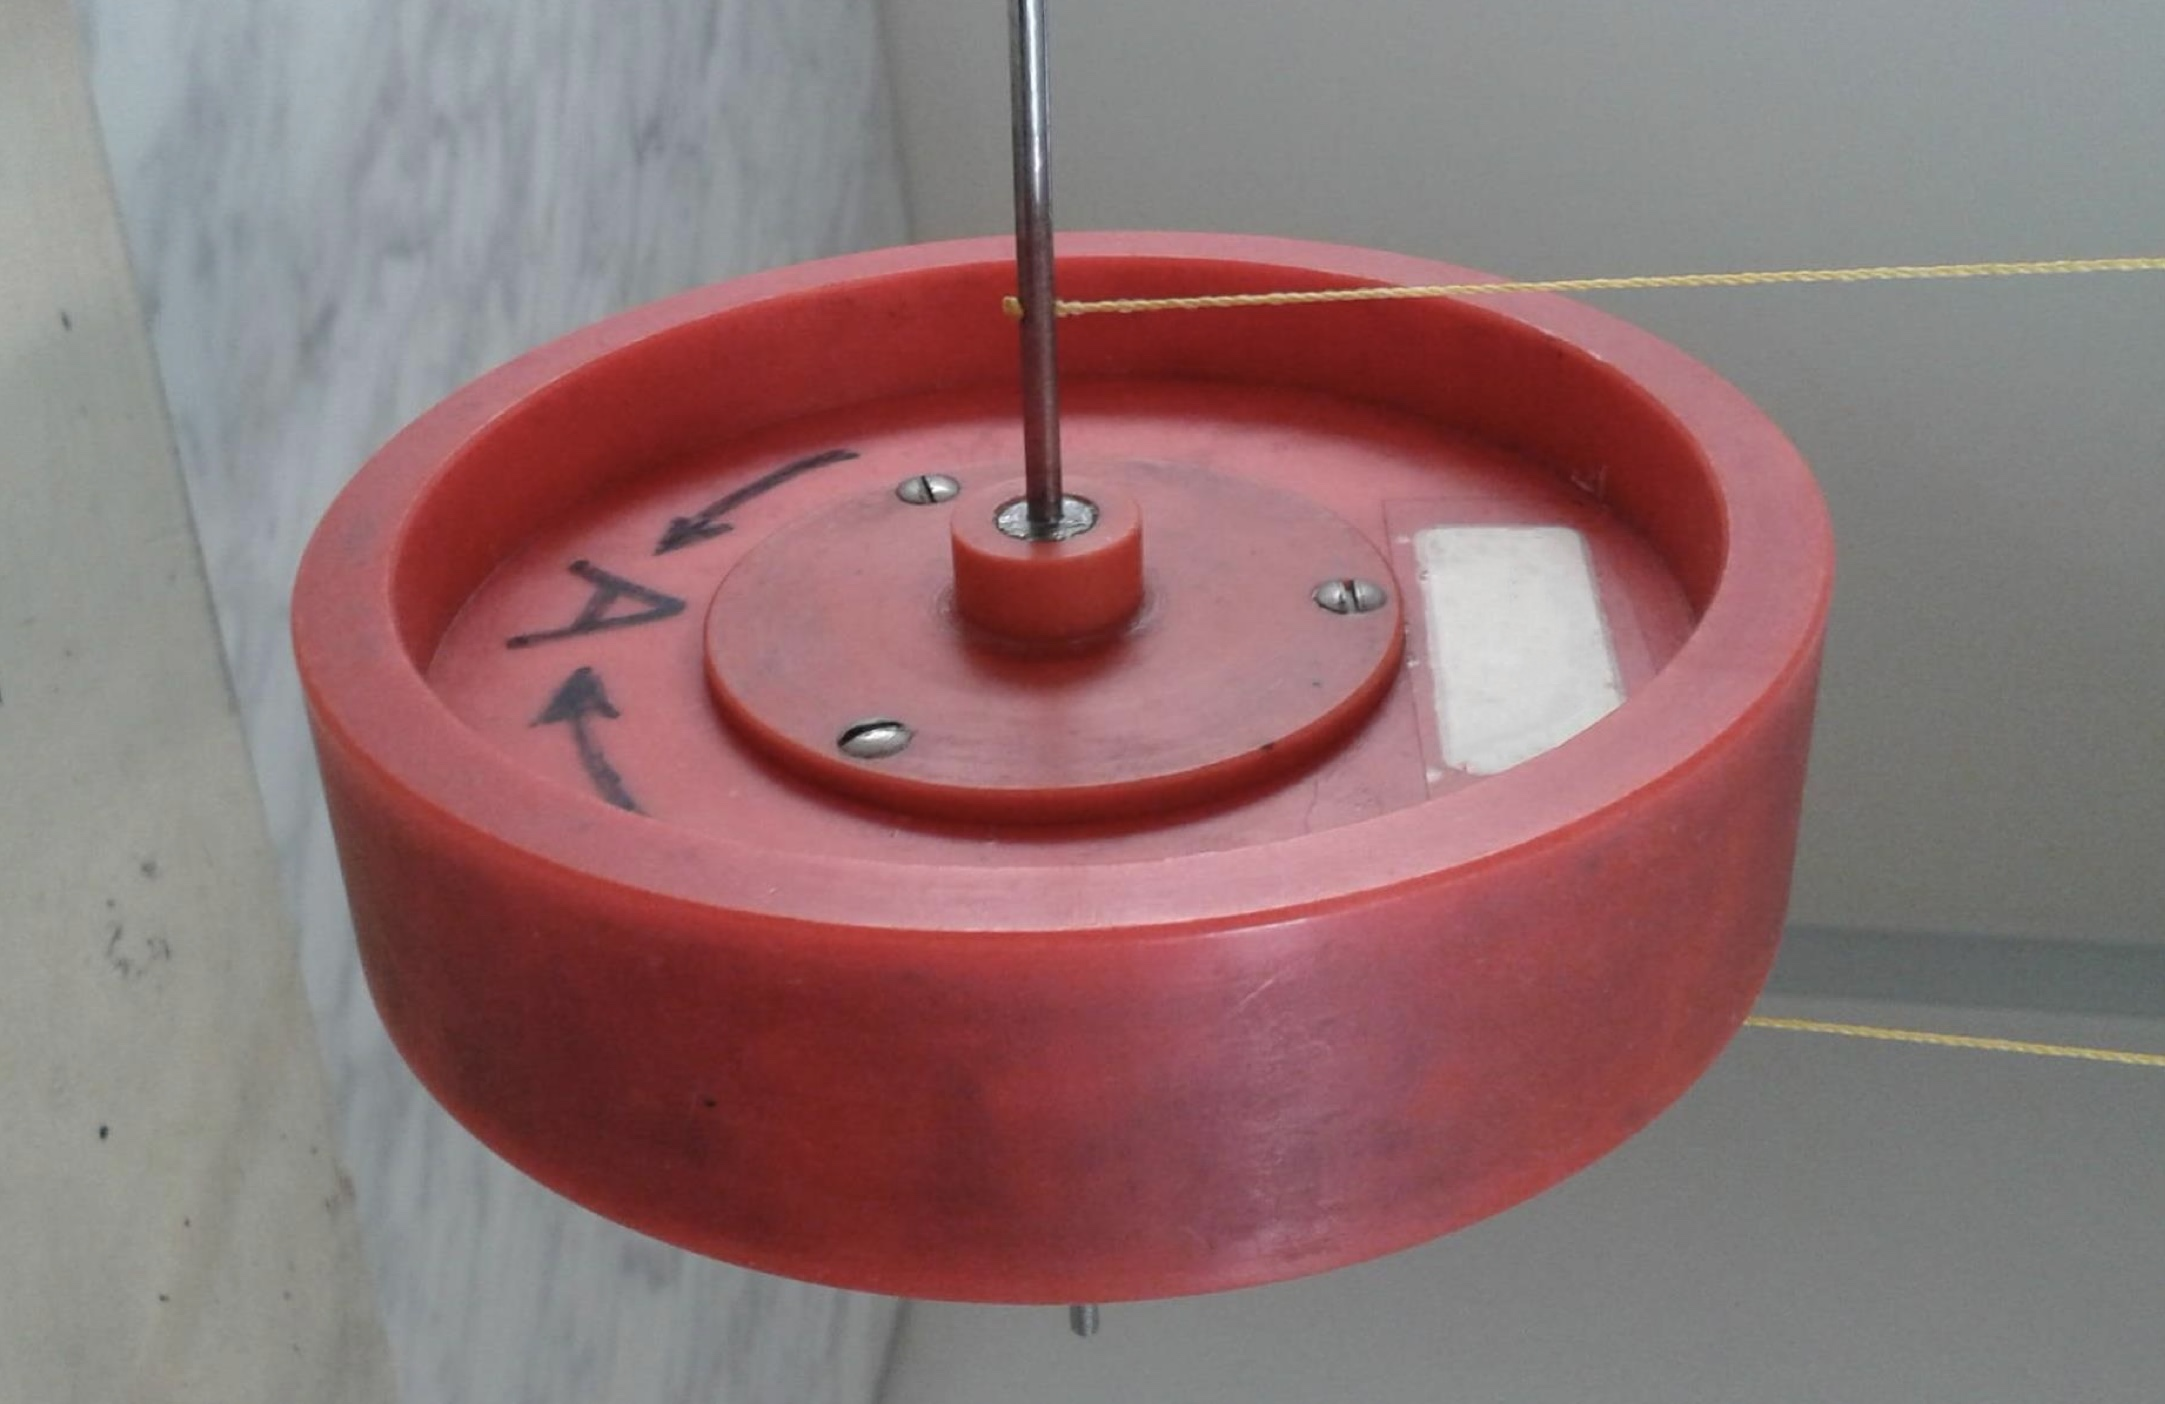
\includegraphics[width=0.70\textwidth]{image/Disco.jpeg}
        \caption[\small Il disco non omogeneo.]{\small Il disco non omogeneo di cui calcolare il momento d'inerzia è composta da quattro toroidi concentrici. Al centro di esso vi è il perno metallico appeso ai due fili del pendolo di Maxwell}
        \label{disco}
    \end{figure}\\
    \item Un \textbf{cronometro digitale} (risoluzione: 0.01 s) di uno smartphone.
    \item Un \textbf{calibro digitale} (risoluzione: 0.01 mm) munito di ganasce da muovere manualmente.
    \item Un \textbf{micrometro manuale} (risoluzione: 0.01 mm) munito di ganasce che vengono mosse da una vite micrometrica, fatta girare manualmente da un tamburo.
    \item Un \textbf{metro a nastro} metallico (risoluzione: 1 mm).
    \begin{figure}[htbp]
        \centering
        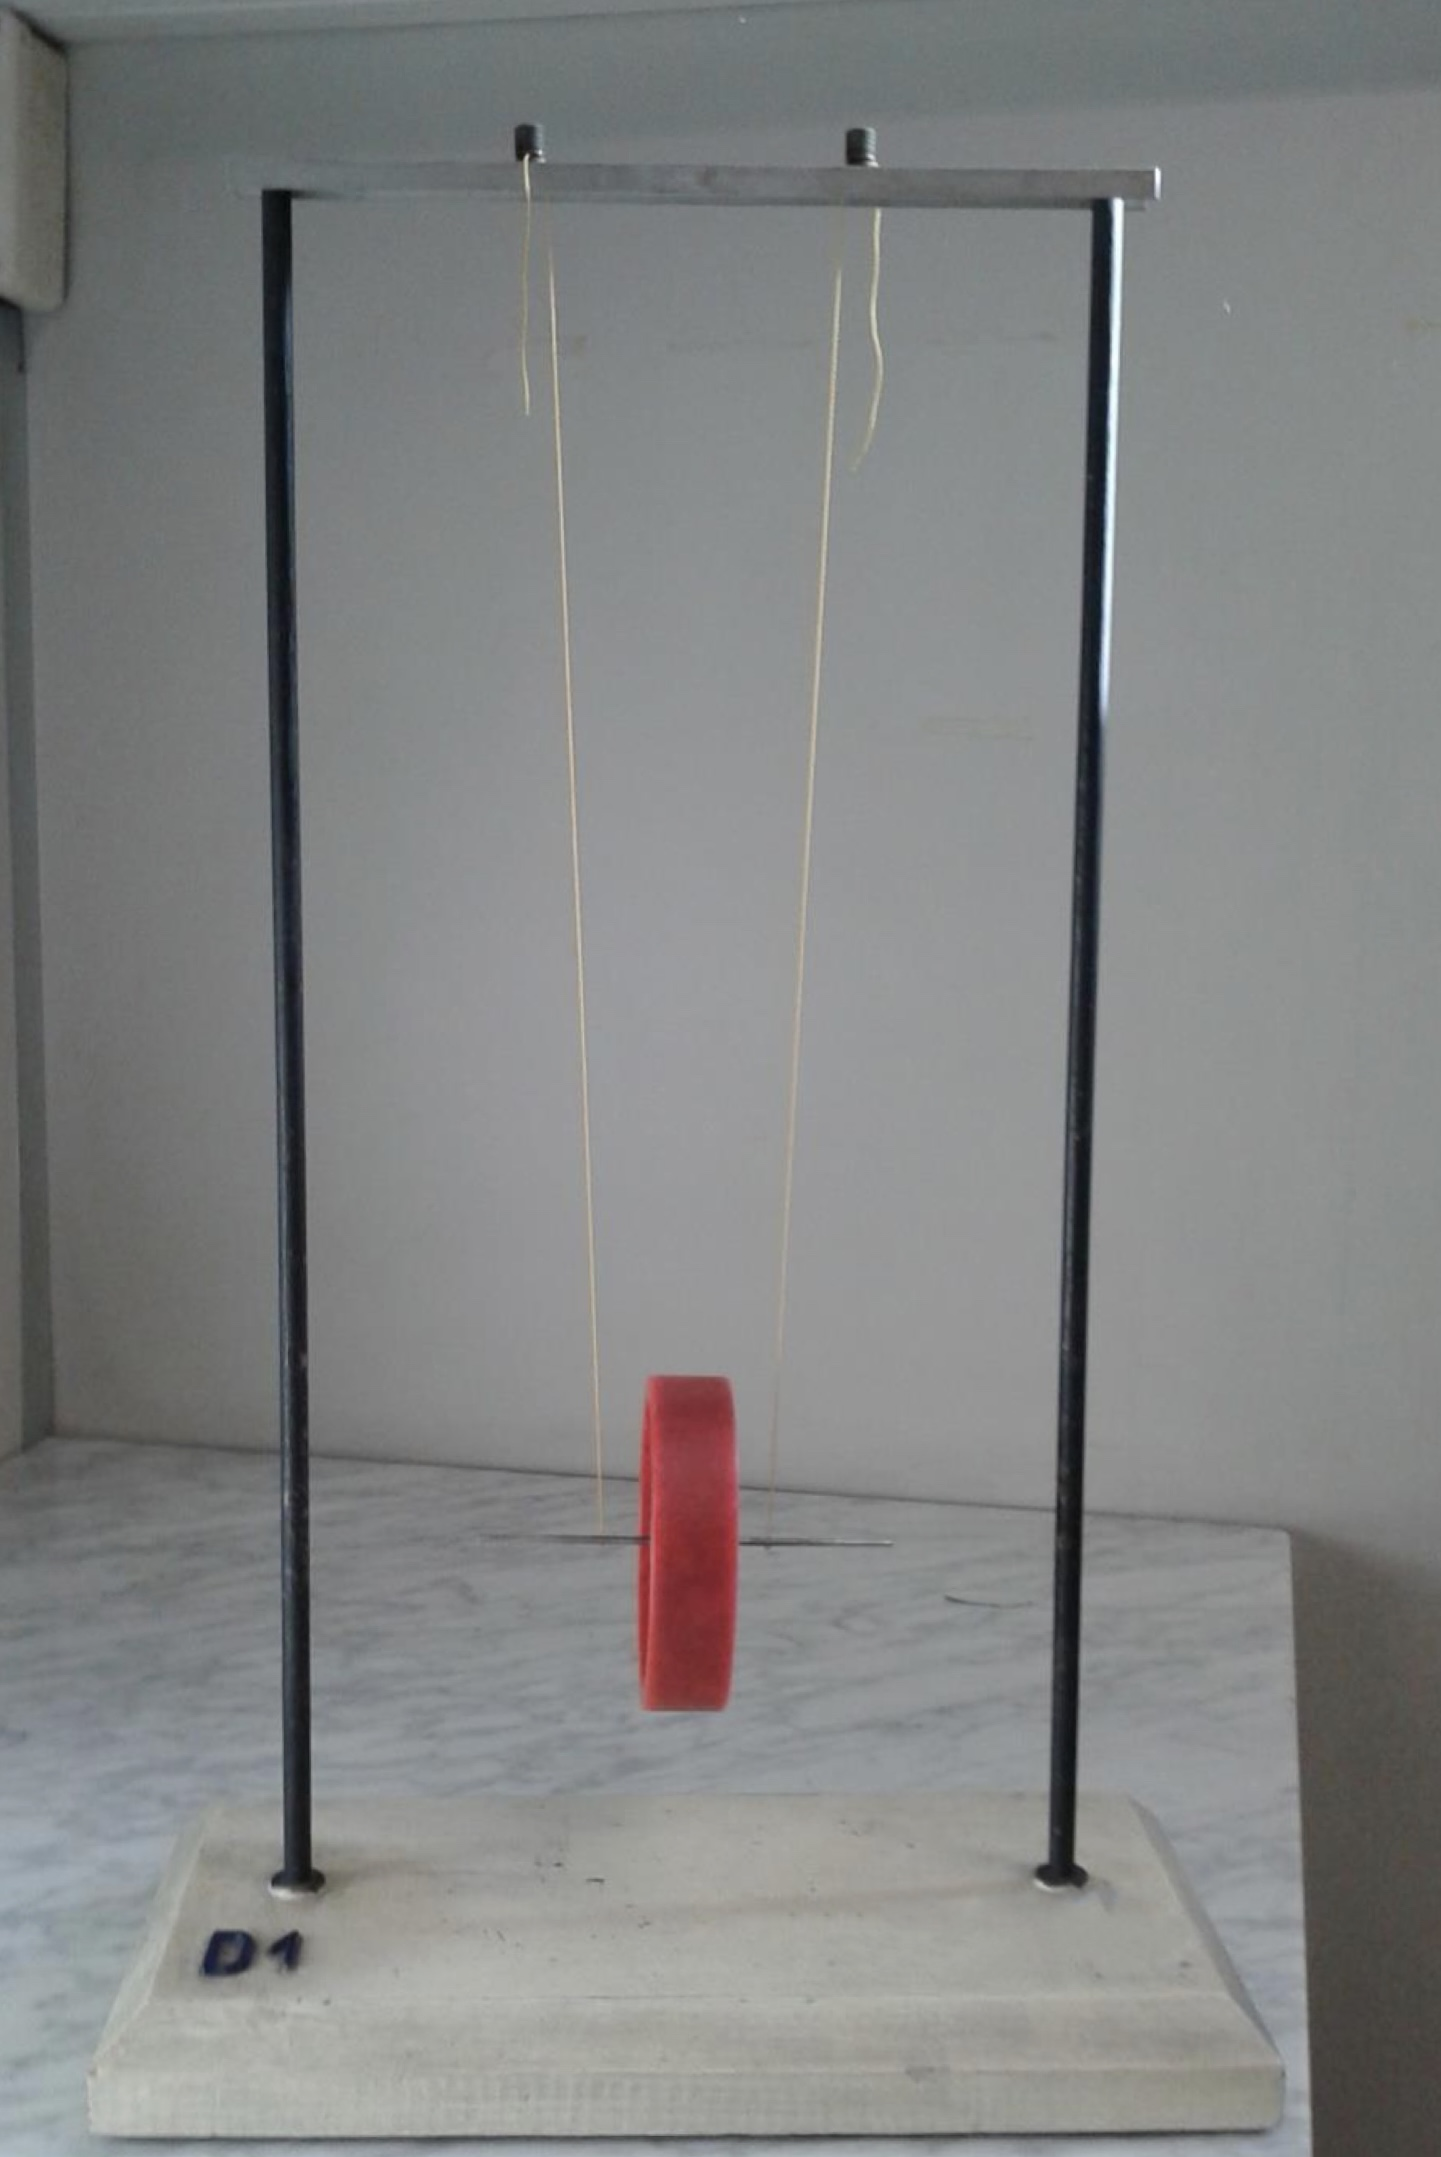
\includegraphics[width=0.65\textwidth]{image/Pendolo_di_Maxwell.jpeg}
        \caption[\small Il pendolo di Maxwell.]{\small Il pendolo di Maxwell con vista frontale: il disco di cui misurare il momento d'inerzia è appeso ai fili che sono fissati all'impalcatura dell'apparato.}
        \label{pendolo_di_maxwel}
    \end{figure}\\
\end{itemize}

%%%%% 1.2 Svolgimento
    \subsection{Svolgimento}
    
    Per misurare il momento d'inerzia si è proceduti per due modi: metodo geometrico e metodo dinamico.

\subsubsection*{Metodo geometrico}

La geometria del disco non omogeneo è stata valutata prendendo misure delle dimensioni dei vari toroidi, numerati per semplicità da 1 a 4 a partire da quello più interno. In Fig. \ref{sezione} è possibile visualizzare la proiezione ortogonale della semisezione assiale del disco.
    \begin{figure}[h]
        \centering
        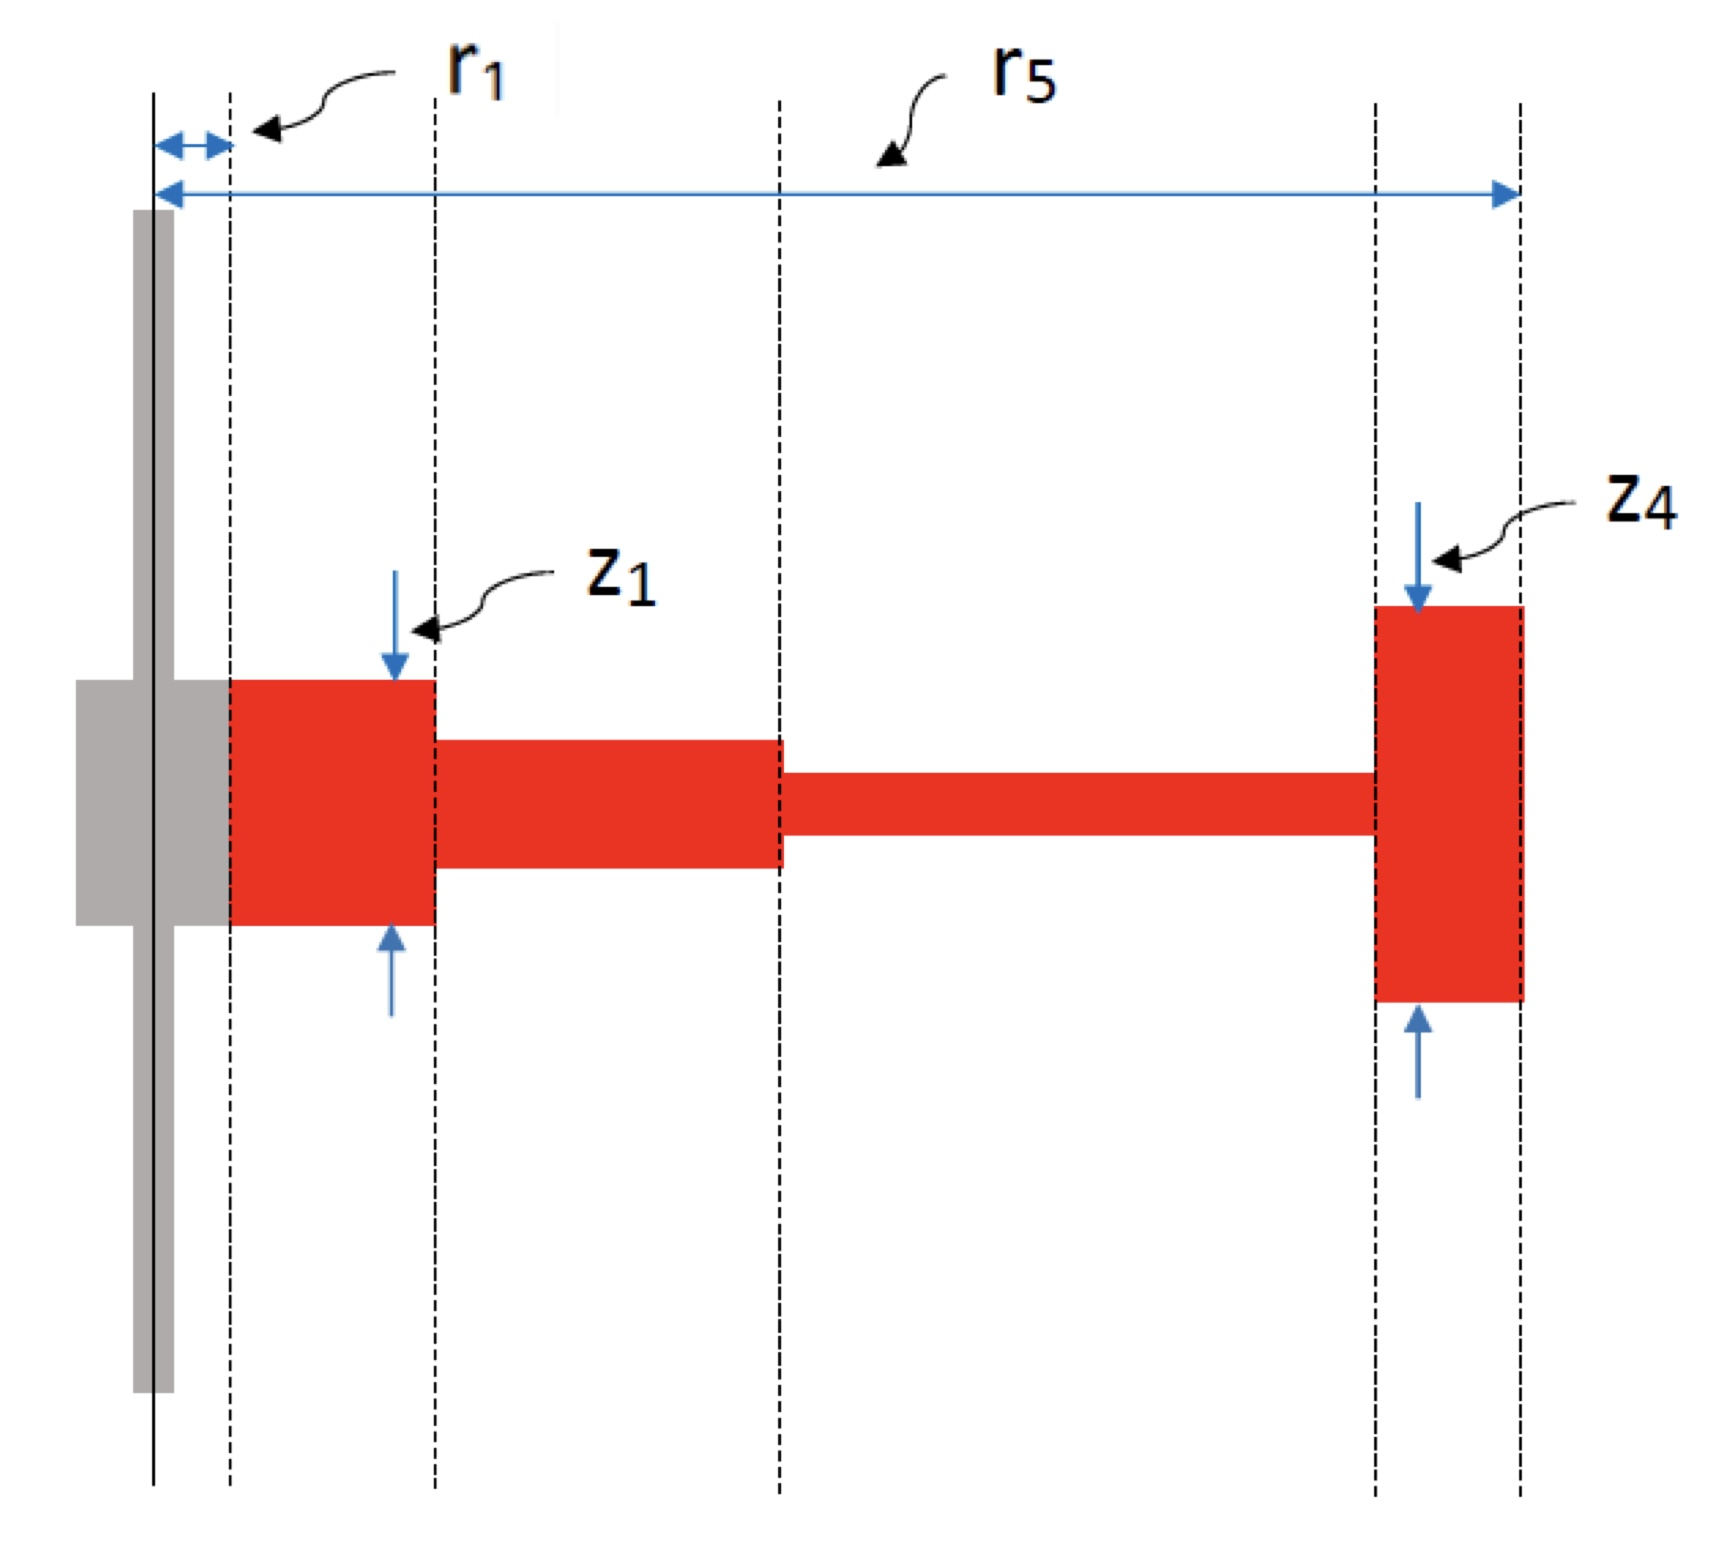
\includegraphics[width=0.6\textwidth]{image/Sezionedisco.jpeg}
        \caption[\small Visualizzazione della semisezione assiale del disco.]{\small Visualizzazione della semisezione assiale del disco. La parte grigia della sezione corrisponde al perno metallico, mentre le parti rosse indicano i toroidi. $r_1$ e $r_5$ sono rispettivamente il raggio interno del primo toroide e quello esterno della quarta, mentre $z_1$ e $z_4$ indicano rispettivamente lo spessore del primo toroide e della quarta.}
        \label{sezione}
    \end{figure}\\
Quindi si è andati a misurare i diametri dei toroidi e i vari spessori con il calibro digitale, mentre per la densità era già data \textit{a priori}.
Per misurare i diametri $d_i$ si sono fatte 3 misure per ogni grandezza, tranne per $d_1$, per il quale si sono fatte 5 misure, perché nell'utilizzo del calibro il luogo in corrispondenza del diametro più interno non aveva punti fissi d'appoggio.\\
Invece per i spessori $z_i$ la situazione è diversa: si può misurare direttamente solo lo spessore più esterno $z_4$, mentre per i restanti, considerando solo una faccia del disco, è stato possibile misurare le tre profondità presenti, numerate da 1 a 3 dall'interno verso l'esterno (Fig. \ref{profondità}). In questo caso sono state fatte quattro misure per ogni grandezza.
    \begin{figure}[htbp]
        \centering
        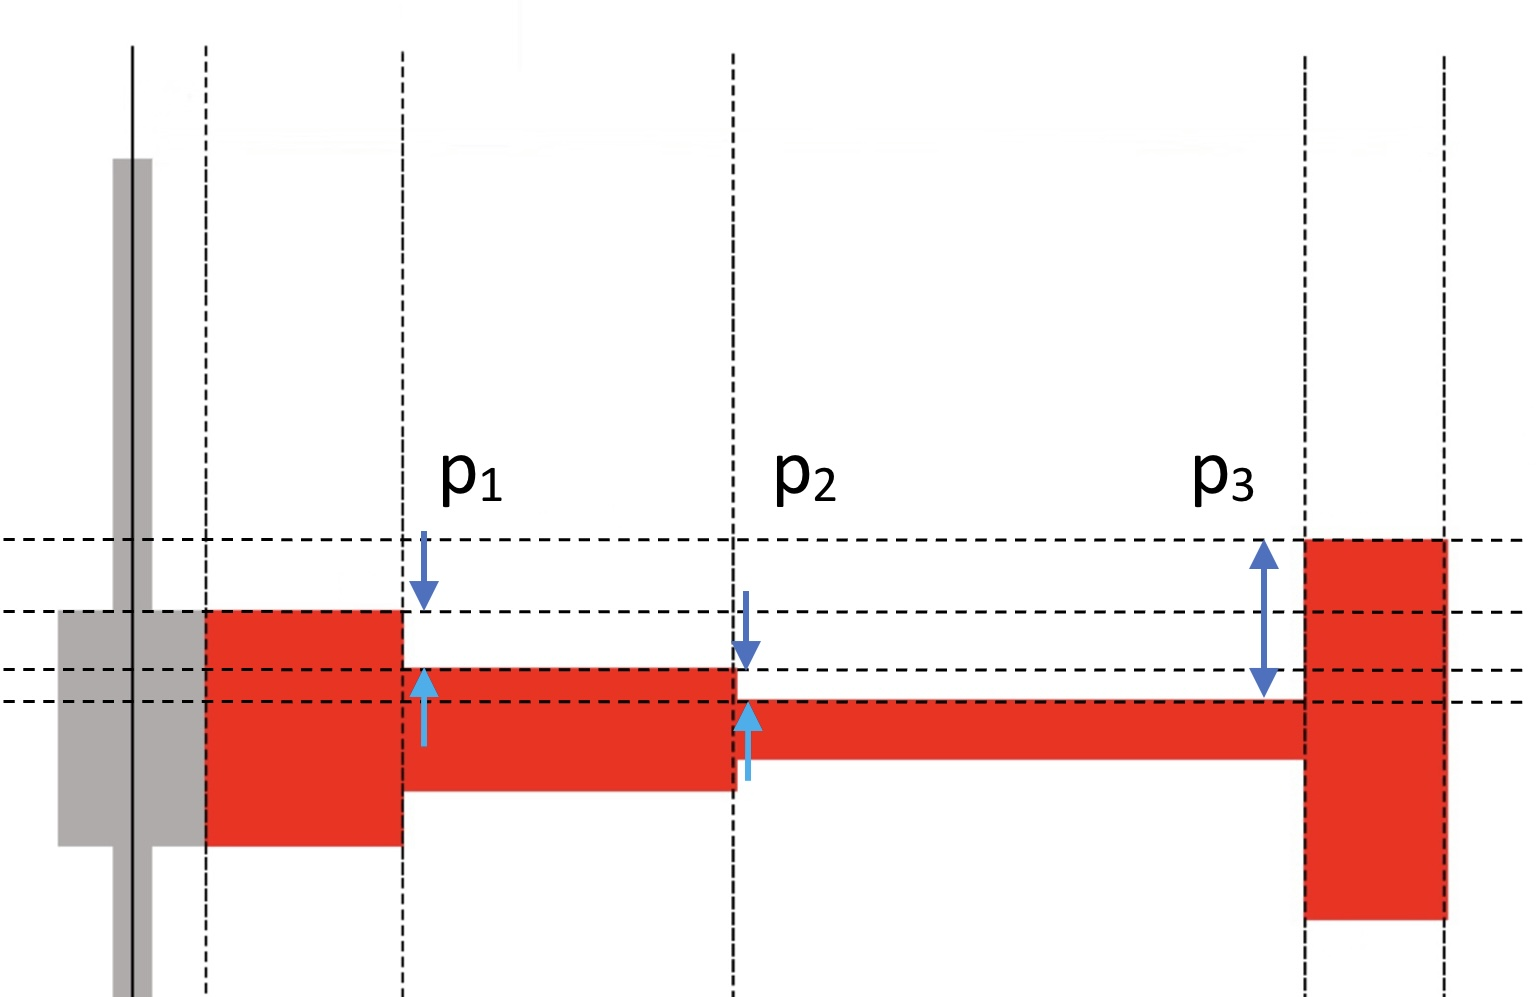
\includegraphics[width=0.75\textwidth]{image/Profondità.jpeg}
        \caption[\small Visualizzazione della semisezione assiale del disco - profondità]{\small Visualizzazione della semisezione assiale del disco. Vengono indicate in particolare le profondità da misurare con il calibro: $p_1$, $p_2$, $p_3$.}
        \label{profondità}
    \end{figure}\\
Per ogni toroide poi si è andati a calcolare il suo momento d'inerzia $I_i$ secondo la formula
$$\displaystyle I_i = \frac{\rho \pi}{32} \cdot z_i (d_{i+1}^4 - d_i^4) $$
con $\rho$ la densità del toroide, $z_i$ lo spessore del toroide $i$, $d_i$ il diametro interno del toroide e $d_{i+1}$ il diametro esterno.\\
Come abbiamo visto, il momento d'inerzia è additiva per oggetti rotanti sullo stesso asse, perciò il momento d'inerzia totale $I_G$ calcolato geometricamente equivale a
\begin{equation} \label{I_G}
    \displaystyle I_G = \sum_{i=1}^4  I_i = \frac{\rho \pi}{32} \cdot \sum_{i=1}^4 z_i (d_{i+1}^4 - d_i^4)
\end{equation}

\subsubsection*{Metodo dinamico}
Per il calcolo del momento d'inerzia ricorrendo per metodo dinamico si è utilizzato il pendolo di Maxwell, perché è necessario il \textbf{tempo di caduta} del disco $t_o$. Per far ciò si è andati ad utilizzare il cronometro digitale.\\
Chiamando per semplicità la posizione iniziale del disco “posizione di quiete", arrotolando il filo attorno il perno metallico, il disco si porta lentamente il alto, fino a raggiungere all'\textbf{altezza massima} $h_o$, misurata 3 volte rispetto alla posizione di quiete con il metro a nastro; lasciando cadere il disco questo assume un moto rototraslatorio uniformemente accelerato verso il basso, fino a raggiungere la posizione di quiete. Il cronometro viene fatto partire dall'instante in cui si lascia il disco e fatto fermare quando raggiunge la posizione di quiete.\\
Visto che la misura di $t_o$ è influenzato dal nostro tempo di reazione, allora si è andati a ripetere  40 volte lo stesso procedimento. Distribuendo le 40 misure in bin da 0.1 s, si è fatto la media per ottenere $t_o$.\\
Inoltre sono state effettuate misure del \textbf{diametro del perno metallico e dei fili}, rispettivamente $d_p$ e $d_f$, attraverso l'utilizzo del micrometro, effettuando 3 misure per ciascuna grandezza.
Per quanto riguarda invece la massa del disco $m$, il valore è stato fornito \textit{a priori}.\\

Ottenuti i parametri si può andare a calcolare il valore del momento d'inerzia del disco $I_D$ mediante metodo dinamico con la seguente formula:
\begin{equation} \label{I_D}
\displaystyle I_D = \frac{m(d_p + d_f)}{8h_o}(gt_o^2+2h_o)
\end{equation}
con $g$ l'accelerazione di gravità terrestre.

\newpage
% 2. Risultati
\section{Risultati}
In questo paragrafo verranno trattati i risultati di misure dirette e misure indirette e metodi con cui si è eseguito l'analisi dei dati
%%%%% 2.1 Acquisizione dati

    \subsection{Acquisizione dati}
    
    %% 2.1 Acquisizioni dati
Qui vengono riportati i valori misurati direttamente per i due metodi.

\subsubsection*{Metodo geometrico}
Per le misure del metodo geometrico è stato fornito direttamente il valore della densità $\rho$ della plastica di cui sono composti i toroidi del disco, e ciò equivale a
$$\rho = (1.36 \pm 0.02) \cdot 10^3 \textrm{ kg/m} ^3$$
Mentre i valori dei diametri $d_i$, delle profondità $p_i$  e di $z_4$ sono riportati in Tab. \ref{diametri_e_spessori}.\\

    \begin{table}[htp]
        \centering
        \begin{tabular}{||c|c|c|c|c||c|c|c||c||}
            \hline \hline
            \multicolumn{9}{||c||}{Misure delle lunghezze per il metodo geometrico (in mm)} \\
            \hline \hline
            $d_1$ & $d_2$ & $d_3$ & $d_4$ & $d_5$ & $p_1$ & $p_2$ & $p_3$ & $z_4$ \\
            \hline
            7.86 & 15.95 & 57.99 & 99.88 & 120.05 & 8.13 & 3.06 & 13.11 & 29.96 \\
            7.82 & 15.93 & 57.99 & 99.89 & 120.03 & 8.17 & 3.06 & 13.16 & 29.95 \\
            7.78 & 15.93 & 57.97 & 99.87 & 120.05 & 7.93 & 3.06 & 13.09 & 29.96 \\
            7.95 &       &       &       &        & 8.17 & 3.16 & 13.19 & 29.95 \\
            7.88 &       &       &       &        &      &      &       &       \\
            \hline \hline 
        \end{tabular}
        \caption[\small Misure delle lunghezze per il metodo geometrico.]{\small I valori riportati in mm delle misure effettuate sui toroidi, in particolare i diametri $d_i$, le profondità $p_i$, e lo spessore del toroide più esterno $z_4$. Da notare come le misure di $d_1$ fluttuino di più rispetto alle altre misure, proprio perché è stato difficile prendere la misura in corrispondenza del diametro più interno.}
        \label{diametri_e_spessori}
    \end{table}

\subsubsection*{Metodo dinamico}
Le 40 misure del tempo vengono riportate su Tab. \ref{tab_tempi_di_caduta}.
    \begin{table}[htp]
        \centering
        \begin{tabular}{||cccccccc||}
            \hline \hline
            \multicolumn{8}{||c||}{Misure del tempo di caduta del disco (in s)} \\
            \hline \hline
            7.31 & 7.41 & 7.39 & 7.49 & 7.32 & 7.56 & 7.42 & 7.69 \\
            7.52 & 7.52 & 7.32 & 7.47 & 7.56 & 7.54 & 7.34 & 7.56 \\
            7.37 & 7.51 & 7.34 & 7.36 & 7.29 & 7.32 & 7.46 & 7.39 \\
            7.39 & 7.37 & 7.39 & 7.24 & 7.29 & 7.57 & 7.41 & 7.37 \\
            7.44 & 7.44 & 7.41 & 7.46 & 7.36 & 7.42 & 7.54 & 7.44 \\
            \hline \hline 
        \end{tabular}
        \caption[\small Misure dei tempi di caduta.]{\small Nella tabella sono riportate i 40 valori del tempo di caduta del disco, in secondi, misurate con il cronometro.}
        \label{tab_tempi_di_caduta}
    \end{table}
Mentre le misure del diametro del filo $d_f$ e del perno metallico $d_p$ e dell'altezza di caduta $h_o$ sono riportate in Tab. \ref{altre_misure}.

    \begin{table}[htp]
        \centering
        \begin{tabular}{||c|c||c||}
            \hline \hline
            $d_f$ [mm] & $d_p$ [mm] & $h_o$ [cm] \\
            \hline
            0.45 & 3.00 & 35.4 \\
            0.40 & 3.02 & 35.4 \\
            0.41 & 3.02 & 35.6 \\
            \hline \hline 
        \end{tabular}
        \caption[\small Misure delle lunghezze per il metodo dinamico.]{\small Le misure del diametro del filo $d_f$ e del perno $d_p$ (in mm), dell'altezza di caduta del disco $h_o$ (in cm).}
        \label{altre_misure}
    \end{table}
\newpage
    
%%%%% 2.2 Elaborazione dati e risultati quantitativi

    \subsection{Elaborazione dati e risultati quantitativi}
    
    %% 2.2 Elaborazione dati e risutati quantitativi
In questo paragrafo si riportano i dati elaborati, il calcolo delle misure indirette e la valutazione degli errori.\\
Per le grandezze per le quali si sono fatte più misure (tranne per il tempo) si è considerata come stima migliore la media, mentre come incertezza la semidispersione delle misure.\\
Nel caso in cui alcune incertezze valutate con la semidispersione siano risultati non sensati rispetto al setup sperimentale (per esempio incertezze troppo basse), allora si è andati a considerare la risoluzione dello strumento come incertezza.

\subsubsection*{Metodo geometrico}
I valori dei diametri $d_i$ sono:
    \begin{align*}
        d_1 &= (7.86 \pm 0.09) \textrm{ mm} \\
        d_2 &= (15.94 \pm 0.01) \textrm{ mm} \\
        d_3 &= (57.98 \pm 0.01) \textrm{ mm} \\
        d_4 &= (99.88 \pm 0.01) \textrm{ mm} \\
        d_5 &= (120.04 \pm 0.01) \textrm{ mm} 
    \end{align*}
Per le profondità $p_i$ e lo spessore del toroide più esterno $z_4$ si riportano i seguenti valori:
    \begin{align*}
        p_1 &= (8.1 \pm 0.1) \textrm{ mm} \\
        p_2 &= (3.09 \pm 0.05) \textrm{ mm} \\
        p_3 &= (13.14 \pm 0.05) \textrm{ mm} \\
        z_4 &= (29.96 \pm 0.01) \textrm{ mm} \\
    \end{align*}
Attraverso un'analisi geometrica della sezione assiale del disco, riportato in Fig. \ref{profondità} a pag. \pageref{profondità}, i spessori dei primi tre toroidi sono risultati:
    \begin{align*}
        z_1 &= (26.1 \pm 0.4) \textrm{ mm} \\
        z_2 &= (9.9 \pm 0.2) \textrm{ mm} \\
        z_3 &= (3.7 \pm 0.1) \textrm{ mm}
    \end{align*}
in cui gli errori sono stati calcolati secondo la propagazione degli errori considerando l'incertezza massima.\\

Per il calcolo del momento d'inerzia, ricorrendo alla formula (\ref{I_G}) a pag. \pageref{I_G}, si è ottenuto il valore di 
$$I_G = 4.91 \cdot 10^{-4} \textrm{ kg} \cdot \textrm{m}^2$$
Per la valutazione dell'errore si è ricorso al metodo della propagazione dell'errore con derivate, procedimento mostrato a App. \ref{errore_I_G} a pag. \pageref{errore_I_G}.\\
Dunque il valore finale di $I_G$ è di
$$I_G = (4.91 \pm 0.08) \cdot 10^{-4} \textrm{ kg} \cdot \textrm{m}^2$$

\subsubsection*{Metodo dinamico}
Per il metodo dinamico il valore della massa del disco era già stato fornito \textit{a priori}: 
$$m = (226.0 \pm 0.5) \textrm{ g}$$
Le misure dell'altezza di caduta, del diametro del perno e del filo sono stati:
\begin{align*}
    h_o &= (35.5 \pm 0.1) \textrm{ cm} \\
    d_p &= (0.42 \pm 0.03) \textrm{ mm} \\
    d_f &= (3.01 \pm 0.01) \textrm{ mm}
\end{align*}
Le misure del tempo di caduta del disco sono state raccolte in bin da 0.1 s, con occorrenze per ogni bin indicato nella Tab. \ref{tab_tempi_di_caduta_2}.
\begin{table}[htp]
    \begin{center}
        \begin{tabular}{||c|c||}
            \hline
            \hline
            \multicolumn{2}{||c||}{Tempi di caduta}\\
            \hline \hline
            tempo [s] & occorrenze \\
            \hline
            7.2 & 1\\
            7.3 & 7\\
            7.4 & 18\\
            7.5 & 9\\
            7.6 & 4\\
            7.7 & 1\\
            \hline
            \hline
        \end{tabular}
    \end{center}
    \caption[\small Tabella di tempi di caduta - occorrenze.]{\small Sono indicati i numeri di occorrenze dei tempi di caduta del disco per bin ampi 0.1 s. Si nota che il valore del tempo di caduta medio è di 7.43 s.}
    \label{tab_tempi_di_caduta_2}
\end{table}\\
Analizzando graficamente i dati della Tab. \ref{tab_tempi_di_caduta_2} si hanno ottenuto due grafici d'istogramma: il primo indica il numero delle occorrenze per bin (Fig. \ref{istogramma_tempi_di_caduta}), il secondo invece indica la frequenza dei valori in ogni bin (Fig. \ref{distribuzione_tempi_di_caduta}).
     \begin{figure}[htbp]
        \centering
        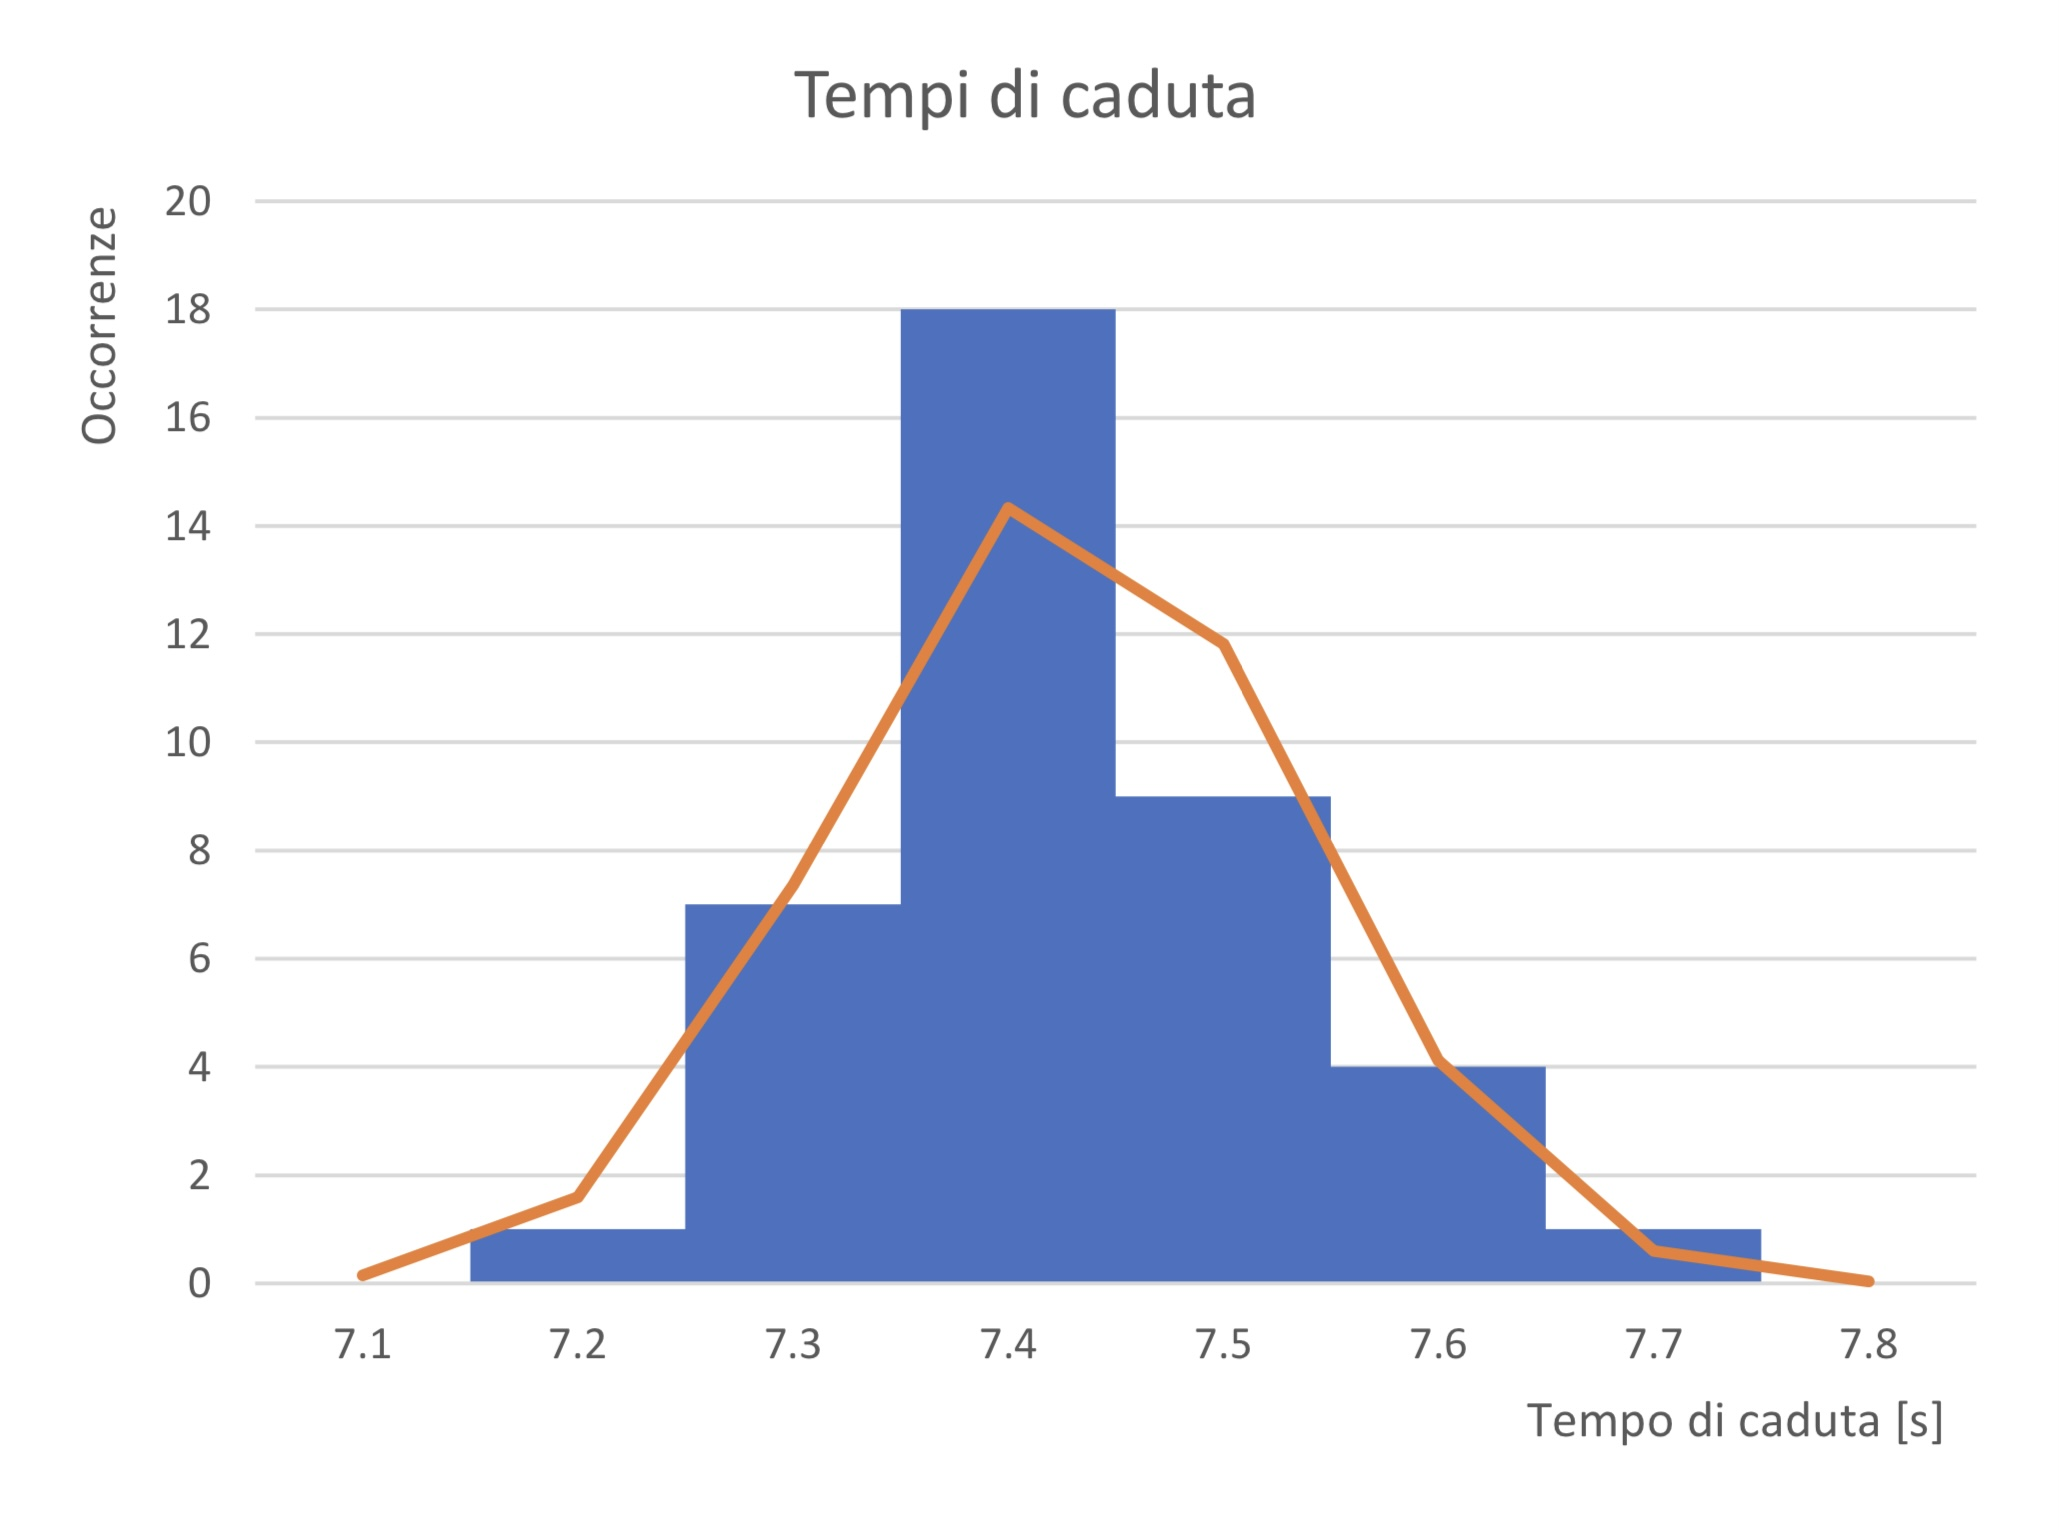
\includegraphics[width=\textwidth]{image/Istogramma_tempi_di_caduta.jpeg}
        \caption[\small L'istogramma del conteggio dei tempi di caduta del disco.]{\small Nell'istogramma sono riportati il numero di occorrenze (sull'asse delle ordinate) in corrispondenza di ogni bin da 0.1 s (sull'asse delle ascisse). Invece la linea spezzata arancione rappresenterebbe il valore atteso secondo la gaussiana con media e deviazione standard calcolato con i dati riportati in Tab. \ref{tab_tempi_di_caduta_2}.}
        \label{istogramma_tempi_di_caduta}
    \end{figure}
    
    \begin{figure}[htbp]
        \centering
        \begin{tikzpicture}[scale = 0.75, every node/.style={scale=0.75}]
\pgfdeclareplotmark{cross} {
\pgfpathmoveto{\pgfpoint{-0.3\pgfplotmarksize}{\pgfplotmarksize}}
\pgfpathlineto{\pgfpoint{+0.3\pgfplotmarksize}{\pgfplotmarksize}}
\pgfpathlineto{\pgfpoint{+0.3\pgfplotmarksize}{0.3\pgfplotmarksize}}
\pgfpathlineto{\pgfpoint{+1\pgfplotmarksize}{0.3\pgfplotmarksize}}
\pgfpathlineto{\pgfpoint{+1\pgfplotmarksize}{-0.3\pgfplotmarksize}}
\pgfpathlineto{\pgfpoint{+0.3\pgfplotmarksize}{-0.3\pgfplotmarksize}}
\pgfpathlineto{\pgfpoint{+0.3\pgfplotmarksize}{-1.\pgfplotmarksize}}
\pgfpathlineto{\pgfpoint{-0.3\pgfplotmarksize}{-1.\pgfplotmarksize}}
\pgfpathlineto{\pgfpoint{-0.3\pgfplotmarksize}{-0.3\pgfplotmarksize}}
\pgfpathlineto{\pgfpoint{-1.\pgfplotmarksize}{-0.3\pgfplotmarksize}}
\pgfpathlineto{\pgfpoint{-1.\pgfplotmarksize}{0.3\pgfplotmarksize}}
\pgfpathlineto{\pgfpoint{-0.3\pgfplotmarksize}{0.3\pgfplotmarksize}}
\pgfpathclose
\pgfusepathqstroke
}
\pgfdeclareplotmark{cross*} {
\pgfpathmoveto{\pgfpoint{-0.3\pgfplotmarksize}{\pgfplotmarksize}}
\pgfpathlineto{\pgfpoint{+0.3\pgfplotmarksize}{\pgfplotmarksize}}
\pgfpathlineto{\pgfpoint{+0.3\pgfplotmarksize}{0.3\pgfplotmarksize}}
\pgfpathlineto{\pgfpoint{+1\pgfplotmarksize}{0.3\pgfplotmarksize}}
\pgfpathlineto{\pgfpoint{+1\pgfplotmarksize}{-0.3\pgfplotmarksize}}
\pgfpathlineto{\pgfpoint{+0.3\pgfplotmarksize}{-0.3\pgfplotmarksize}}
\pgfpathlineto{\pgfpoint{+0.3\pgfplotmarksize}{-1.\pgfplotmarksize}}
\pgfpathlineto{\pgfpoint{-0.3\pgfplotmarksize}{-1.\pgfplotmarksize}}
\pgfpathlineto{\pgfpoint{-0.3\pgfplotmarksize}{-0.3\pgfplotmarksize}}
\pgfpathlineto{\pgfpoint{-1.\pgfplotmarksize}{-0.3\pgfplotmarksize}}
\pgfpathlineto{\pgfpoint{-1.\pgfplotmarksize}{0.3\pgfplotmarksize}}
\pgfpathlineto{\pgfpoint{-0.3\pgfplotmarksize}{0.3\pgfplotmarksize}}
\pgfpathclose
\pgfusepathqfillstroke
}
\pgfdeclareplotmark{newstar} {
\pgfpathmoveto{\pgfqpoint{0pt}{\pgfplotmarksize}}
\pgfpathlineto{\pgfqpointpolar{44}{0.5\pgfplotmarksize}}
\pgfpathlineto{\pgfqpointpolar{18}{\pgfplotmarksize}}
\pgfpathlineto{\pgfqpointpolar{-20}{0.5\pgfplotmarksize}}
\pgfpathlineto{\pgfqpointpolar{-54}{\pgfplotmarksize}}
\pgfpathlineto{\pgfqpointpolar{-90}{0.5\pgfplotmarksize}}
\pgfpathlineto{\pgfqpointpolar{234}{\pgfplotmarksize}}
\pgfpathlineto{\pgfqpointpolar{198}{0.5\pgfplotmarksize}}
\pgfpathlineto{\pgfqpointpolar{162}{\pgfplotmarksize}}
\pgfpathlineto{\pgfqpointpolar{134}{0.5\pgfplotmarksize}}
\pgfpathclose
\pgfusepathqstroke
}
\pgfdeclareplotmark{newstar*} {
\pgfpathmoveto{\pgfqpoint{0pt}{\pgfplotmarksize}}
\pgfpathlineto{\pgfqpointpolar{44}{0.5\pgfplotmarksize}}
\pgfpathlineto{\pgfqpointpolar{18}{\pgfplotmarksize}}
\pgfpathlineto{\pgfqpointpolar{-20}{0.5\pgfplotmarksize}}
\pgfpathlineto{\pgfqpointpolar{-54}{\pgfplotmarksize}}
\pgfpathlineto{\pgfqpointpolar{-90}{0.5\pgfplotmarksize}}
\pgfpathlineto{\pgfqpointpolar{234}{\pgfplotmarksize}}
\pgfpathlineto{\pgfqpointpolar{198}{0.5\pgfplotmarksize}}
\pgfpathlineto{\pgfqpointpolar{162}{\pgfplotmarksize}}
\pgfpathlineto{\pgfqpointpolar{134}{0.5\pgfplotmarksize}}
\pgfpathclose
\pgfusepathqfillstroke
}
\definecolor{c}{rgb}{1,1,1};
\draw [color=c, fill=c] (0,0) rectangle (20,13.5817);
\draw [color=c, fill=c] (2,1.35817) rectangle (18,12.2235);
\definecolor{c}{rgb}{0,0,0};
\draw [c,line width=0.9] (2,1.35817) -- (2,12.2235) -- (18,12.2235) -- (18,1.35817) -- (2,1.35817);
\definecolor{c}{rgb}{1,1,1};
\draw [color=c, fill=c] (2,1.35817) rectangle (18,12.2235);
\definecolor{c}{rgb}{0,0,0};
\draw [c,line width=0.9] (2,1.35817) -- (2,12.2235) -- (18,12.2235) -- (18,1.35817) -- (2,1.35817);
\draw [c,line width=0.9] (2,1.35817) -- (18,1.35817);
\draw [c,dash pattern=on 0.80pt off 1.60pt ,line width=0.9] (3,12.2235) -- (3,1.35817);
\draw [c,dash pattern=on 0.80pt off 1.60pt ,line width=0.9] (5,12.2235) -- (5,1.35817);
\draw [c,dash pattern=on 0.80pt off 1.60pt ,line width=0.9] (7,12.2235) -- (7,1.35817);
\draw [c,dash pattern=on 0.80pt off 1.60pt ,line width=0.9] (9,12.2235) -- (9,1.35817);
\draw [c,dash pattern=on 0.80pt off 1.60pt ,line width=0.9] (11,12.2235) -- (11,1.35817);
\draw [c,dash pattern=on 0.80pt off 1.60pt ,line width=0.9] (13,12.2235) -- (13,1.35817);
\draw [c,dash pattern=on 0.80pt off 1.60pt ,line width=0.9] (15,12.2235) -- (15,1.35817);
\draw [c,dash pattern=on 0.80pt off 1.60pt ,line width=0.9] (17,12.2235) -- (17,1.35817);
\draw [c,dash pattern=on 0.80pt off 1.60pt ,line width=0.9] (3,12.2235) -- (3,1.35817);
\draw [c,dash pattern=on 0.80pt off 1.60pt ,line width=0.9] (17,12.2235) -- (17,1.35817);
\draw [c,line width=0.9] (2,1.35817) -- (2,12.2235);
\draw [c,dash pattern=on 0.80pt off 1.60pt ,line width=0.9] (18,1.35817) -- (2,1.35817);
\draw [c,dash pattern=on 0.80pt off 1.60pt ,line width=0.9] (18,2.50794) -- (2,2.50794);
\draw [c,dash pattern=on 0.80pt off 1.60pt ,line width=0.9] (18,3.65771) -- (2,3.65771);
\draw [c,dash pattern=on 0.80pt off 1.60pt ,line width=0.9] (18,4.80748) -- (2,4.80748);
\draw [c,dash pattern=on 0.80pt off 1.60pt ,line width=0.9] (18,5.95725) -- (2,5.95725);
\draw [c,dash pattern=on 0.80pt off 1.60pt ,line width=0.9] (18,7.10702) -- (2,7.10702);
\draw [c,dash pattern=on 0.80pt off 1.60pt ,line width=0.9] (18,8.25679) -- (2,8.25679);
\draw [c,dash pattern=on 0.80pt off 1.60pt ,line width=0.9] (18,9.40656) -- (2,9.40656);
\draw [c,dash pattern=on 0.80pt off 1.60pt ,line width=0.9] (18,10.5563) -- (2,10.5563);
\draw [c,dash pattern=on 0.80pt off 1.60pt ,line width=0.9] (18,11.7061) -- (2,11.7061);
\draw [c,dash pattern=on 0.80pt off 1.60pt ,line width=0.9] (18,11.7061) -- (2,11.7061);
\definecolor{c}{rgb}{0,0.4,0.8};
\draw [c, fill=c] (2,1.35817) -- (2,1.35817) -- (4,1.35817) -- (4,1.93305) -- (6,1.93305) -- (6,5.38236) -- (8,5.38236) -- (8,11.7061) -- (10,11.7061) -- (10,6.53213) -- (12,6.53213) -- (12,3.65771) -- (14,3.65771) -- (14,1.93305) -- (16,1.93305) --
 (16,1.35817) -- (18,1.35817) -- (18,1.35817);
\definecolor{c}{rgb}{0,0,0.6};
\draw [c,line width=0.9] (2,1.35817) -- (4,1.35817) -- (4,1.93305) -- (6,1.93305) -- (6,5.38236) -- (8,5.38236) -- (8,11.7061) -- (10,11.7061) -- (10,6.53213) -- (12,6.53213) -- (12,3.65771) -- (14,3.65771) -- (14,1.93305) -- (16,1.93305) --
 (16,1.35817) -- (18,1.35817);
\definecolor{c}{rgb}{0,0,0};
\draw [c,line width=0.9] (2,1.35817) -- (18,1.35817);
\draw [c,line width=0.9] (3,1.68413) -- (3,1.35817);
\draw [c,line width=0.9] (3.4,1.52115) -- (3.4,1.35817);
\draw [c,line width=0.9] (3.8,1.52115) -- (3.8,1.35817);
\draw [c,line width=0.9] (4.2,1.52115) -- (4.2,1.35817);
\draw [c,line width=0.9] (4.6,1.52115) -- (4.6,1.35817);
\draw [c,line width=0.9] (5,1.68413) -- (5,1.35817);
\draw [c,line width=0.9] (5.4,1.52115) -- (5.4,1.35817);
\draw [c,line width=0.9] (5.8,1.52115) -- (5.8,1.35817);
\draw [c,line width=0.9] (6.2,1.52115) -- (6.2,1.35817);
\draw [c,line width=0.9] (6.6,1.52115) -- (6.6,1.35817);
\draw [c,line width=0.9] (7,1.68413) -- (7,1.35817);
\draw [c,line width=0.9] (7.4,1.52115) -- (7.4,1.35817);
\draw [c,line width=0.9] (7.8,1.52115) -- (7.8,1.35817);
\draw [c,line width=0.9] (8.2,1.52115) -- (8.2,1.35817);
\draw [c,line width=0.9] (8.6,1.52115) -- (8.6,1.35817);
\draw [c,line width=0.9] (9,1.68413) -- (9,1.35817);
\draw [c,line width=0.9] (9.4,1.52115) -- (9.4,1.35817);
\draw [c,line width=0.9] (9.8,1.52115) -- (9.8,1.35817);
\draw [c,line width=0.9] (10.2,1.52115) -- (10.2,1.35817);
\draw [c,line width=0.9] (10.6,1.52115) -- (10.6,1.35817);
\draw [c,line width=0.9] (11,1.68413) -- (11,1.35817);
\draw [c,line width=0.9] (11.4,1.52115) -- (11.4,1.35817);
\draw [c,line width=0.9] (11.8,1.52115) -- (11.8,1.35817);
\draw [c,line width=0.9] (12.2,1.52115) -- (12.2,1.35817);
\draw [c,line width=0.9] (12.6,1.52115) -- (12.6,1.35817);
\draw [c,line width=0.9] (13,1.68413) -- (13,1.35817);
\draw [c,line width=0.9] (13.4,1.52115) -- (13.4,1.35817);
\draw [c,line width=0.9] (13.8,1.52115) -- (13.8,1.35817);
\draw [c,line width=0.9] (14.2,1.52115) -- (14.2,1.35817);
\draw [c,line width=0.9] (14.6,1.52115) -- (14.6,1.35817);
\draw [c,line width=0.9] (15,1.68413) -- (15,1.35817);
\draw [c,line width=0.9] (15.4,1.52115) -- (15.4,1.35817);
\draw [c,line width=0.9] (15.8,1.52115) -- (15.8,1.35817);
\draw [c,line width=0.9] (16.2,1.52115) -- (16.2,1.35817);
\draw [c,line width=0.9] (16.6,1.52115) -- (16.6,1.35817);
\draw [c,line width=0.9] (17,1.68413) -- (17,1.35817);
\draw [c,line width=0.9] (3,1.68413) -- (3,1.35817);
\draw [c,line width=0.9] (2.6,1.52115) -- (2.6,1.35817);
\draw [c,line width=0.9] (2.2,1.52115) -- (2.2,1.35817);
\draw [c,line width=0.9] (17,1.68413) -- (17,1.35817);
\draw [c,line width=0.9] (17.4,1.52115) -- (17.4,1.35817);
\draw [c,line width=0.9] (17.8,1.52115) -- (17.8,1.35817);
\draw [anchor=base] (3,0.909971) node[scale=1.08185, color=c, rotate=0]{7.1};
\draw [anchor=base] (5,0.909971) node[scale=1.08185, color=c, rotate=0]{7.2};
\draw [anchor=base] (7,0.909971) node[scale=1.08185, color=c, rotate=0]{7.3};
\draw [anchor=base] (9,0.909971) node[scale=1.08185, color=c, rotate=0]{7.4};
\draw [anchor=base] (11,0.909971) node[scale=1.08185, color=c, rotate=0]{7.5};
\draw [anchor=base] (13,0.909971) node[scale=1.08185, color=c, rotate=0]{7.6};
\draw [anchor=base] (15,0.909971) node[scale=1.08185, color=c, rotate=0]{7.7};
\draw [anchor=base] (17,0.909971) node[scale=1.08185, color=c, rotate=0]{7.8};
\draw [anchor= east] (18,0.597593) node[scale=1.08185, color=c, rotate=0]{tempo [s]};
\draw [c,line width=0.9] (2,1.35817) -- (2,12.2235);
\draw [c,line width=0.9] (2.48,1.35817) -- (2,1.35817);
\draw [c,line width=0.9] (2.24,1.58812) -- (2,1.58812);
\draw [c,line width=0.9] (2.24,1.81807) -- (2,1.81807);
\draw [c,line width=0.9] (2.24,2.04803) -- (2,2.04803);
\draw [c,line width=0.9] (2.24,2.27798) -- (2,2.27798);
\draw [c,line width=0.9] (2.48,2.50794) -- (2,2.50794);
\draw [c,line width=0.9] (2.24,2.73789) -- (2,2.73789);
\draw [c,line width=0.9] (2.24,2.96784) -- (2,2.96784);
\draw [c,line width=0.9] (2.24,3.1978) -- (2,3.1978);
\draw [c,line width=0.9] (2.24,3.42775) -- (2,3.42775);
\draw [c,line width=0.9] (2.48,3.65771) -- (2,3.65771);
\draw [c,line width=0.9] (2.24,3.88766) -- (2,3.88766);
\draw [c,line width=0.9] (2.24,4.11762) -- (2,4.11762);
\draw [c,line width=0.9] (2.24,4.34757) -- (2,4.34757);
\draw [c,line width=0.9] (2.24,4.57752) -- (2,4.57752);
\draw [c,line width=0.9] (2.48,4.80748) -- (2,4.80748);
\draw [c,line width=0.9] (2.24,5.03743) -- (2,5.03743);
\draw [c,line width=0.9] (2.24,5.26739) -- (2,5.26739);
\draw [c,line width=0.9] (2.24,5.49734) -- (2,5.49734);
\draw [c,line width=0.9] (2.24,5.72729) -- (2,5.72729);
\draw [c,line width=0.9] (2.48,5.95725) -- (2,5.95725);
\draw [c,line width=0.9] (2.24,6.1872) -- (2,6.1872);
\draw [c,line width=0.9] (2.24,6.41716) -- (2,6.41716);
\draw [c,line width=0.9] (2.24,6.64711) -- (2,6.64711);
\draw [c,line width=0.9] (2.24,6.87706) -- (2,6.87706);
\draw [c,line width=0.9] (2.48,7.10702) -- (2,7.10702);
\draw [c,line width=0.9] (2.24,7.33697) -- (2,7.33697);
\draw [c,line width=0.9] (2.24,7.56693) -- (2,7.56693);
\draw [c,line width=0.9] (2.24,7.79688) -- (2,7.79688);
\draw [c,line width=0.9] (2.24,8.02683) -- (2,8.02683);
\draw [c,line width=0.9] (2.48,8.25679) -- (2,8.25679);
\draw [c,line width=0.9] (2.24,8.48674) -- (2,8.48674);
\draw [c,line width=0.9] (2.24,8.7167) -- (2,8.7167);
\draw [c,line width=0.9] (2.24,8.94665) -- (2,8.94665);
\draw [c,line width=0.9] (2.24,9.1766) -- (2,9.1766);
\draw [c,line width=0.9] (2.48,9.40656) -- (2,9.40656);
\draw [c,line width=0.9] (2.24,9.63651) -- (2,9.63651);
\draw [c,line width=0.9] (2.24,9.86647) -- (2,9.86647);
\draw [c,line width=0.9] (2.24,10.0964) -- (2,10.0964);
\draw [c,line width=0.9] (2.24,10.3264) -- (2,10.3264);
\draw [c,line width=0.9] (2.48,10.5563) -- (2,10.5563);
\draw [c,line width=0.9] (2.24,10.7863) -- (2,10.7863);
\draw [c,line width=0.9] (2.24,11.0162) -- (2,11.0162);
\draw [c,line width=0.9] (2.24,11.2462) -- (2,11.2462);
\draw [c,line width=0.9] (2.24,11.4761) -- (2,11.4761);
\draw [c,line width=0.9] (2.48,11.7061) -- (2,11.7061);
\draw [c,line width=0.9] (2.48,11.7061) -- (2,11.7061);
\draw [c,line width=0.9] (2.24,11.9361) -- (2,11.9361);
\draw [c,line width=0.9] (2.24,12.166) -- (2,12.166);
\draw [anchor= east] (1.9,1.35817) node[scale=1.08185, color=c, rotate=0]{0};
\draw [anchor= east] (1.9,2.50794) node[scale=1.08185, color=c, rotate=0]{0.5};
\draw [anchor= east] (1.9,3.65771) node[scale=1.08185, color=c, rotate=0]{1};
\draw [anchor= east] (1.9,4.80748) node[scale=1.08185, color=c, rotate=0]{1.5};
\draw [anchor= east] (1.9,5.95725) node[scale=1.08185, color=c, rotate=0]{2};
\draw [anchor= east] (1.9,7.10702) node[scale=1.08185, color=c, rotate=0]{2.5};
\draw [anchor= east] (1.9,8.25679) node[scale=1.08185, color=c, rotate=0]{3};
\draw [anchor= east] (1.9,9.40656) node[scale=1.08185, color=c, rotate=0]{3.5};
\draw [anchor= east] (1.9,10.5563) node[scale=1.08185, color=c, rotate=0]{4};
\draw [anchor= east] (1.9,11.7061) node[scale=1.08185, color=c, rotate=0]{4.5};
\draw [anchor= east] (0.698281,12.2235) node[scale=1.08185, color=c, rotate=90]{$\Phi [s^{-1}]$};
\definecolor{c}{rgb}{1,1,1};
\draw [color=c, fill=c] (15.6,10.5258) rectangle (19.6,12.6989);
\definecolor{c}{rgb}{0,0,0};
\draw [c,line width=0.9] (15.6,10.5258) -- (19.6,10.5258);
\draw [c,line width=0.9] (19.6,10.5258) -- (19.6,12.6989);
\draw [c,line width=0.9] (19.6,12.6989) -- (15.6,12.6989);
\draw [c,line width=0.9] (15.6,12.6989) -- (15.6,10.5258);
\draw (17.6,12.4272) node[scale=1.08185, color=c, rotate=0]{histo};
\draw [c,line width=0.9] (15.6,12.1556) -- (19.6,12.1556);
\draw [anchor= west] (15.8,11.884) node[scale=1.08185, color=c, rotate=0]{Entries };
\draw [anchor= east] (19.4,11.884) node[scale=1.08185, color=c, rotate=0]{ 8};
\draw [anchor= west] (15.8,11.3407) node[scale=1.08185, color=c, rotate=0]{Mean  };
\draw [anchor= east] (19.4,11.3407) node[scale=1.08185, color=c, rotate=0]{  7.427};
\draw [anchor= west] (15.8,10.7974) node[scale=1.08185, color=c, rotate=0]{Std Dev   };
\draw [anchor= east] (19.4,10.7974) node[scale=1.08185, color=c, rotate=0]{ 0.1024};
\definecolor{c}{rgb}{0,0.6,0};
\draw [c,line width=1.8] (2.08,1.37172) -- (2.24,1.376) -- (2.4,1.3815) -- (2.56,1.38851) -- (2.72,1.3974) -- (2.88,1.40859) -- (3.04,1.42258) -- (3.2,1.43997) -- (3.36,1.46143) -- (3.52,1.48776) -- (3.68,1.51983) -- (3.84,1.55864) -- (4,1.6053) --
 (4.16,1.66101) -- (4.32,1.72709) -- (4.48,1.80491) -- (4.64,1.89594) -- (4.8,2.00168) -- (4.96,2.12364) -- (5.12,2.26332) -- (5.28,2.42215) -- (5.44,2.60143) -- (5.6,2.80231) -- (5.76,3.0257) -- (5.92,3.27223) -- (6.08,3.54218) -- (6.24,3.83543) --
 (6.4,4.15139) -- (6.56,4.48898) -- (6.72,4.84656) -- (6.88,5.22195) -- (7.04,5.61235) -- (7.2,6.01443) -- (7.36,6.4243) -- (7.52,6.83757) -- (7.68,7.24942) -- (7.84,7.65466) -- (8,8.04789) -- (8.16,8.42353) -- (8.32,8.77603) -- (8.48,9.09994) --
 (8.64,9.39009) -- (8.8,9.64171) -- (8.96,9.85056) -- (9.12,10.0131) -- (9.28,10.1264) -- (9.44,10.1885) -- (9.6,10.1984) -- (9.76,10.1558) -- (9.92,10.0614);
\draw [c,line width=1.8] (9.92,10.0614) -- (10.08,9.9171) -- (10.24,9.72525) -- (10.4,9.4892) -- (10.56,9.21296) -- (10.72,8.90113) -- (10.88,8.55872) -- (11.04,8.19111) -- (11.2,7.80382) -- (11.36,7.40244) -- (11.52,6.99245) -- (11.68,6.57913) --
 (11.84,6.16744) -- (12,5.76196) -- (12.16,5.36675) -- (12.32,4.98538) -- (12.48,4.62083) -- (12.64,4.27552) -- (12.8,3.95129) -- (12.96,3.64943) -- (13.12,3.37071) -- (13.28,3.11541) -- (13.44,2.8834) -- (13.6,2.67418) -- (13.76,2.48692) --
 (13.92,2.32057) -- (14.08,2.17387) -- (14.24,2.04543) -- (14.4,1.93378) -- (14.56,1.83741) -- (14.72,1.75481) -- (14.88,1.6845) -- (15.04,1.62506) -- (15.2,1.57516) -- (15.36,1.53354) -- (15.52,1.49906) -- (15.68,1.47069) -- (15.84,1.4475) --
 (16,1.42867) -- (16.16,1.41348) -- (16.32,1.4013) -- (16.48,1.39161) -- (16.64,1.38394) -- (16.8,1.37791) -- (16.96,1.3732) -- (17.12,1.36955) -- (17.28,1.36673) -- (17.44,1.36457) -- (17.6,1.36293) -- (17.76,1.36169);
\draw [c,line width=1.8] (17.76,1.36169) -- (17.92,1.36075);
\definecolor{c}{rgb}{0,0,0};
\draw (10,13.1011) node[scale=1.52731, color=c, rotate=0]{Distribuzione dei tempi di caduta};
\end{tikzpicture}

        \caption[\small L'istogramma della distribuzione dei tempi di caduta del disco.]{\small Istogramma riportante la distribuzione della frequenza delle misure relative ai tempi di caduta. La curva verde rappresenta la gaussiana che rappresenterebbe al meglio la PDF associata alla distribuzione.}
        \label{distribuzione_tempi_di_caduta}
    \end{figure}

Con queste informazioni si è andati a calcolare il valore del tempo medio di caduta come $t_o$:
$$t_o = 7.43 \textrm{ s}$$
Mentre come valore dell'incertezza del tempo di caduta si è preso in considerazione la deviazione standard della media delle misure, di cui riportiamo la formula in App. \ref{SD} a pag. \pageref{SD}. Tuttavia, dato il numero ridotto di campionamenti, si considera anche un fattore di copertura $k=3$. Si riporta il valore dell'incertezza di $t_o$.
$$\Delta t_o = 0.05 \textrm{ s}$$
Perciò il valore finale di $t_o$ è
$$\displaystyle t_o = (7.43 \pm 0.05) \textrm{ s}$$\\

Ottenuto tutti valori necessari per la valutazione del momento d'inerzia calcolato per via dinamica $I_D$, con $ g = 9.81$ m/s$^2$, si da il seguente risultato, secondo la formula (\ref{I_D}) a pag. \pageref{I_D}:
$$ I_D = 5.1 \cdot 10^{-4} \textrm{ kg} \cdot \textrm{m}^2$$

Per la valutazione dell'incertezza di $I_D$ si è usato la propagazione degli errori per incertezze massime (riportiamo la formula in App. \ref{errore_I_D} a pag. \pageref{errore_I_D}). Perciò il valore finale di $I_D$ è di 
$$ I_D = (5.1 \pm 0.2) \cdot 10^{-4} \textrm{ kg} \cdot \textrm{m}^2$$

% conclusione -----------------------------------
\section*{Conclusione}
\addcontentsline{toc}{section}{Conclusione}
% Conclusione

Dai risultati ottenuti si confrontano i valori di $I_D$ e $I_G$:

\begin{align*}
    I_G &= (4.91 \pm 0.08) \cdot 10^{-4} \textrm{ kg} \cdot \textrm{m}^2\\
    I_D &= (5.1 \pm 0.2) \cdot 10^{-4} \textrm{ kg} \cdot \textrm{m}^2 \\
\end{align*}
Per cui si può affermare che i valori sono compatibili entro l'errore.\\

Si osserva che $I_G$ è minore di $I_D$. Questo potrebbe essere causato dal non considerare il momento d'inerzia del cilindro metallico. Ma si scopre subito che trascurare la parte metallica è giustificata, perché il suo raggio è molto piccolo. Infatti, facendo una stima, sapendo che la densità di un metallo $\rho_{m}$ è tipicamente di 8 g/cm$^3$ (come il ferro, l'acciaio, rame...), considerando $r_m = d_1/2$ come raggio e $z_1$ come spessore, allora il suo momento d'inerzia è
$$I_m = \frac{1}{2} m_m r_m^2 = \frac{\rho_m \pi}{32} z_1 d_1^4 \approx 8 \cdot 10^{-8} \textrm{ kg} \cdot \textrm{m}^2$$
che rappresenta circa il 0.016\% rispetto a $I_m$. Si evince che la discrepanza è probabilmente dovuta ad altri fattori.\\

I risultati ottenuti comunque hanno senso dal punto di vista fisico: se il disco fosse stato ripieno, o omogeneo, questa avrebbe avuto più massa e quindi anche più momento d'inerzia (vista l'additività). Infatti, facendo un veloce calcolo, considerato un disco con stessa densità $\rho$, diametro $d_5$ e spessore $z_4$, allora il suo momento d'inerzia $I'$ sarebbe stato di
$$I' = \frac{\rho \pi}{32} z_4 d_5^4 \approx 8 \cdot 10^{-4} \textrm{ kg} \cdot \textrm{m}^2$$
ossia quasi il doppio del disco non omogeneo.

%Documento realizzato in \LaTeX, sul sito di %Overleaf$^{\textrm{\cite{overleaf}}}$. Le fonti utilizzati in %fisica sono $^{\textrm{\cite{libroditerza}}}$, %$^{\textrm{\cite{librodiquarta}}}$, %$^{\textrm{\cite{librodiquinta}}}$, %$^{\textrm{\cite{librodiwilliam}}}$ e %$^{\textrm{\cite{tesidilaurea}}}$. Le fonti utilizzati per %matematica sono $^{\textrm{\cite{librodimate1}}}$ e %$^{\textrm{\cite{librodimate2}}}$.
\newpage

% indice
\tableofcontents

% elenco delle figure
\listoffigures
% elenco delle tabelle
\listoftables
\newpage

% bibliografia
\printbibliography[nottype=online, title=Bibliografia]
% sitografia
%\printbibliography[type=online, title=Sitografia]

\newpage

\renewcommand{\appendixpagename}{Appendici}
\renewcommand{\appendixtocname}{Appendici}
\appendix
\appendixpage
\addappheadtotoc

\section{Valutazione dell'incertezza di $I_G$}
 \label{errore_I_G}
L'incertezza del valore del momento d'inerzia $\Delta I_G$ è valutato secondo il metodo della propagazione degli errori con derivate$^{\textrm{\cite{statistica}}}$.
Quindi, ricorrendo alla formula (\ref{I_G}),
    \begin{align*}
        \displaystyle \Delta I_G & = \left|\frac{\partial I_G}{\partial \rho}\right|\Delta \rho + \sum_{i=1}^5 \left|\frac{\partial I_G}{\partial d_i}\right|\Delta d_i + \sum_{i=1}^4 \left|\frac{\partial I_G}{\partial z_i}\right|\Delta z_i \\
        & = \frac{I_G}{\rho} \Delta \rho + \frac{\rho \pi}{8} \left[ \left(z_1 d_1^3 \Delta d_1 + z_4d_5^3 \Delta d_5\right) + \sum_{1=2}^4 \left( d_i^3 |z_i - z_{i-1}|\Delta d_i \right)\right] + \sum_{i=1}^4 \left( \frac{I_i}{z_i} \Delta z_i \right)
    \end{align*}
    
\section{Deviazione standard della media di $t_o$} \label{SD}

Per la valutazione dell'incertezza di $t_o$, lo si valuta come la deviazione standard della media dei valori di $t_o$ e si è utilizzato, insieme ad un fattore di copertura $k$, la seguente formula:
$$\displaystyle \Delta t_o = k \sigma_{\bar{t_o}} = k \cdot \sqrt{\frac{\displaystyle \sum_{i=1}^N (t_i - \bar{t_o})^2}{N(N-1)}}$$
valevole per un serie di $N$ misure $t_i$, con $\Bar{t_o}$ come valore medio.

\section{Valutazione dell'incertezza di $I_D$} \label{errore_I_D}
L'errore di $I_D$ è calcolato secondo la propagazione degli errore per incertezza massima:

$$\displaystyle \frac{\Delta I_D}{I_D} = \frac{\Delta m}{m} + 2\frac{(\Delta d_f + \Delta d_p)}{d_f + d_p} + \frac{\Delta h_o}{h_o} + 2\frac{\Delta t_o}{t_o}$$

\end{document}
